\documentclass[13pt]{beamer}
% \usepackage{natslides}
\mode<presentation>{\usetheme{Copenhagen}}
%\setbeameroption{previous slide on second screen}
\usepackage{pgfpages}
% \setbeameroption{show notes on second screen}
\setbeamerfont{note page}{size=\footnotesize}
\usepackage{graphicx}
\usepackage[english]{babel}
\usepackage[utf8x]{inputenc}
\usepackage{verbatim}
\usepackage{fancyvrb}
\usepackage{textcomp}
\usepackage{enumerate}
\usepackage{mysty}
\usepackage{subfigure}
\usepackage{float}
\usepackage{tabu}
\usepackage{color}
\usepackage{colortbl}
\usepackage{teximporter}
\usepackage{listings}
\usepackage[algoruled,shortend]{algorithm2e}


\newcommand{\abc}{\textsc{abc}}
\newcommand{\abcdt}{\textsc{abc::dt}}
\newcommand{\abcpt}{\abc{} processing tool}
\newcommand{\unix}{\textsc{unix}}
\newcommand{\midi}{\textsc{midi}}
\newcommand{\abcmtops}{\texttt{abcm2ps}}
\newcommand{\abctomidi}{\texttt{abc2midi}}
\newcommand{\abcdtrule}{\abcdt{} \emph{rule}}
\newcommand{\abcdtrules}{\abcdt{} \emph{rules}}
\newcommand{\dt}{\emph{dt}}
\newcommand{\toabc}{\emph{toabc}}
\newcommand{\wcabc}{\texttt{wc\_abc}}

\fvset{fontsize=\footnotesize,[commandchars=\\\{\}]}


\institute{
	\vspace{-.5cm}
	\begin{figure}
		\centering
	   \includegraphics[width=.15\textwidth]{img/eeng}
	\end{figure}
	\vspace{-0.9cm}
	\begin{center}
		Informatics Engineering MSc\\
		University of Minho
	\end{center}
}
\author[Bruno Azevedo, \texttt{azevedo.252@gmail.com}]{Bruno Azevedo\\\texttt{azevedo.252@gmail.com}}

\title{A Toolkit for Music Processing and Analysis}
\date{\small{September 2013}}
\begin{document}

\inlinepin

\begin{frame}[plain]
	\begin{center}
	\maketitle
	\end{center}
	\addtocounter{framenumber}{-1}
\end{frame}

\note{
Bom dia, o meu nome é Bruno Azevedo e venho apresentar a minha dissertação de mestrado intitulada A
Toolkit for Music Processing and Analysis.
Vou começar por fazer uma contextualização do trabalho desenvolvido.
}

\begin{frame}[fragile]{\abc{} music notation}
  \begin{block}{\abc{}}
    Textual music notation standard
  \end{block}
  \pause

  \begin{exampleblock}{Example}
  \begin{Verbatim}
  X:1
  T:Verbum caro factum est
  M:3/4
  L:1/8
  K:G
  G4 G2 | G4 F2 |A4 A2 | B4 z2|
  w: Ver- bum|ca- ro|fac- tum|est|
  \end{Verbatim}

	\vspace{-.75cm}
  \begin{figure}[htb]
    \centering
    \includegraphics[width=\textwidth,clip=true, trim = 0mm 10mm 40mm 10mm]{img/abc.pdf}
  \end{figure}
	\vspace{-14cm}
  \end{exampleblock}

% \inline_makefileg[rankdir=1,scale=0.5]{
% LaTeX: Pdf Midi
% Pdf: abc
%     abcm2ps
% Midi: abc
%     abc2midi
% }
\end{frame}


\note[itemize]{
\item O ABC é um standard textual de notação musical. [NEXT]
\item Este possui uma síntaxe simples e compacta e é capaz de produzir partituras reais
através de ferramentas externas como o abcm2ps que gera partituras em PostScript ou SVG.
}

\definecolor{Gray}{gray}{0.85}

\begin{frame}{\unix{} metaphor}
\begin{block}{\unix{} philosophy}
Creating simple and efficient tools, which tackle only one problem at a time.
\end{block}
\pause
\begin{center}
  \everyrow{\pause}
  \begin{tabular}{|p{4.4cm}p{5.5cm}|}
    \hline
    \rowcolor{Gray}
    \unix{} & $\Rightarrow$ \abc{} \\
    \hline
    \hline
    Simple single-task tools
    & $\Rightarrow$ Simple single-task tools
    \\
    \hline

    \hline
    Universal type: text stream
    & $\Rightarrow$ \abc{} stream
    \\
    \hline

    \hline
    Compositionality
    & $\Rightarrow$ Compositionality
    \\
    \hline

    \hline
    Development language: \textsc{C}
    & $\Rightarrow$ \abcdt{}
    \\
    \hline

    \hline
    cat, paste, wc, ...
    & $\Rightarrow$ cat\_abc, paste\_abc, wc\_abc, ...
    \\
    \hline
  \end{tabular}
\end{center}
\end{frame}

\note[itemize]{
\item A Filosofia Unix baseia-se no princípio de criar ferramentas simples e eficientes que lidam
apenas com um problema e quando esta é aplicada à realidade \abc{} obtém-se as seguintes normas:
[NEXT]
\item O conceito de criação de ferramentas simples mantém-se.
\item O \abc{}, que é texto, é o tipo universal
\item o que permite articular resultados entre ferramentas.
\item Para facilitar a criação de novas ferramentas, criou-se uma linguagem de desenvolvimento, o
\abcdt{}.
\item E algumas funcionalidades presentes em ferramentas \unix{} podem ser mapeadas para a realidade
\abc{}. Por exemplo o cat, paste, wc, etc...
}

\begin{frame}{\abc{} toolkit and \abcdt{}}
  \pause
  \begin{block}{\abc{} toolkit}
    \begin{itemize}
      \item simple \abcpt{}s
      \item deal with real life \abc{}
      \item aid in musical tasks
    \end{itemize}
  \end{block}
  \pause
  \begin{block}{\abcdt{}}
    \begin{itemize}
      \item rule-based DSL
      \item surgical processing
      \item compact specification
      \item rich embedding mechanisms (Perl)
      \item \abc{} oriented
    \end{itemize}
  \end{block}
\end{frame}

\note[itemize]{
\item tookit: Atualmente, existem diversas soluções para processar \abc{}, no entanto, existe sempre
a necessidade de se fazer um processamento mais personalizado. [NEXT] Por isso, surgiu a necessidade
de criar um toolkit composto por ferramentas simples que lidam com \abc{} real e auxiliam em
diversas tarefas musicais.
\item abcdt: Para além disso, para que seja possível criar, de uma forma fácil e compacta, novas
ferramentas, é necessário um sistema simples que permita especificar o que é cada ferramenta faz.
[NEXT] Então criou-se o \abcdt{}, uma DSL baseada em regras que permite fazer um processamento
cirúrgico e que tem uma especificação compacta embutida em Perl e orientada para \abc{}.
}

%TODO validar titulo
\begin{frame}{Main work}
  \begin{enumerate}
    \item Internal Music Representation
    \item \abcpt{}s and \abcdt{}
    \item \abcdt{} by example
    \item Conclusions
    \item Future Work
  \end{enumerate}
\end{frame}

\note[itemize]{
  \item Depois de uma breve contextualização, passo a apresentar o trabalho realizado;
  % \item Vou apresentar 3 estruturas para representação interna de música;
  \item Vou apresentar a estrutura utilizada para representar internamente uma música;
  \item De seguida, explico a estrutura de uma ferramenta que processa \abc{} e a linguagem
  desenvolvida para facilitar a criação de novas ferramentas, o \abcdt{};
  \item Depois apresento algumas ferramentas criadas através da mesma;
  \item E finalmente, retiro algumas conclusões sobre o trabalho realizado
  \item e faço um levantamento do trabalho futuro.
}

\begin{frame}{Internal Music Representation}
% \setbeamercovered{invisible}
% \pause
  \begin{block}{Part-wise}
    score $\rightarrow$ part*\\
    part $\rightarrow$ (voice, abc\_element*)\\
    \begin{itemize}
      \item melodic studies
    \end{itemize}
  \end{block}
% \pause
  \begin{block}{Time-wise}
    score $\rightarrow$ harmonic\_moment*\\
    harmonic\_moment $\rightarrow$ (time\_offset, voice, abc\_element)*\\
    \begin{itemize}
      \item harmonic studies
    \end{itemize}
  \end{block}
% \pause
%   \only<2-4>{
  % \begin{block}{Source-wise}
  %   score $\rightarrow$ (abc\_element , context)*\\
  %   context $\rightarrow$ (current\_time, current\_voice, ...)
  %   \begin{itemize}
  %     \item generic processing and \abc{} rewriting
  %   \end{itemize}
  % \end{block}
  % }
  % \only<5>{
  \begin{exampleblock}{Source-wise}
    score $\rightarrow$ (abc\_element , context)*\\
    context $\rightarrow$ (current\_time, current\_voice, ...)
    \begin{itemize}
      \item generic processing and \abc{} rewriting
    \end{itemize}
  \end{exampleblock}
  % }
\end{frame}

\note[itemize]{
\item Foram estudadas várias estruturas para representar internamente uma música. A representação
escolhida para ser utilizada nas ferramentas foi a representação source-wise.
\item Que expressa uma música tal como é lida da fonte e que, juntamente com o contexto
(ou seja, informação contextual relativa a cada elemento, como o tempo decorrido, a voz a que
pertence, entre outros), é mais adequada para um processamento genérico, assim como para a reescrita
de \abc{}, já que a ordem dos elementos é preservada.

% \item Foram sugeridas três estruturas possíveis para representar internamente informação musical:
% [NEXT]
% \item A representação part-wise expressa uma música por parte, sendo adequada para estudos
% melódicos, já que permite obter diretamente todos os elementos \abc{} pertencentes a uma parte.
% [NEXT]
% \item A time-wise expressa uma música por momento harmónico, isto é, pelo offset do tempo decorrido
% até àquele momento. Esta é adequada para estudos harmónicos, já que permite obter diretamente todos os
% elementos musicais que ocorrem num momento específico no tempo. [NEXT]
% \item A source-wise expressa uma música tal como é lida da fonte e que, juntamente com o contexto
% (ou seja, informação contextual relativa a cada elemento, como o tempo decorrido, a voz a que
% pertence, entre outros), é mais adequada para um processamento genérico, assim como para a reescrita
% de \abc{}, já que a ordem dos elementos é preservada. [NEXT]
% \item Esta foi a estrutura escolhida para representar internamente uma música.
}

\begin{frame}{\abcpt{}s and \abcdt{}}
  An \abcpt{} follows a traditional compiler's structure:
  \begin{enumerate}
    \item Parse \abc{} input
    \item Transform the generated representation
    \item Generate the output
  \end{enumerate}

	\vspace{-.55cm}
  \begin{figure}[htb]
    \centering
    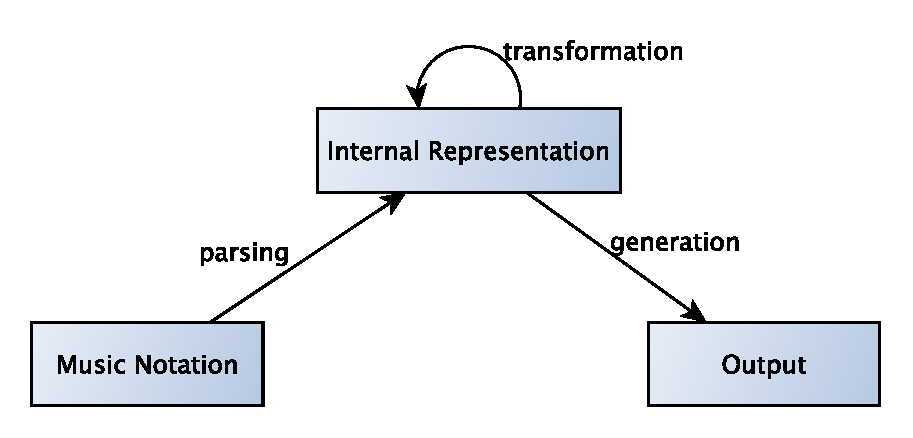
\includegraphics[width=0.8\textwidth]{../img/abc_dt.pdf}
  \end{figure}
  \pause
	\vspace{-.55cm}
  \abcdt{} $\rightarrow$ a DSL (Perl embedded) which allows to create \abcpt{}s in a simple and compact way.
\end{frame}

\note{
Uma típica ferramenta que processa \abc{} segue a estrutura de um compilador tradicional, ou seja:

\begin{enumerate}
  \item O parser gera uma representação interna
  \item A representação interna é transformada
  \item E depois é gerado um output a partir da representação transformada
\end{enumerate}

[NEXT]\\
Para simplificar a criação de novas ferramentas foi criada a DSL \abcdt{}. A descrição do seu
processador vai ser feita utilizando a estrutura apresentada como guia.
}

\begin{frame}{1) Parse \abc{} input stage}
  \begin{block}{Parser}
    \begin{itemize}
      \item Extracted from \abcmtops{}
      \item Common to every \abcpt{}
      \item Its generated IR is source-wise
    \end{itemize}
  \end{block}
  \pause
  \begin{figure}[htb]
    \centering
    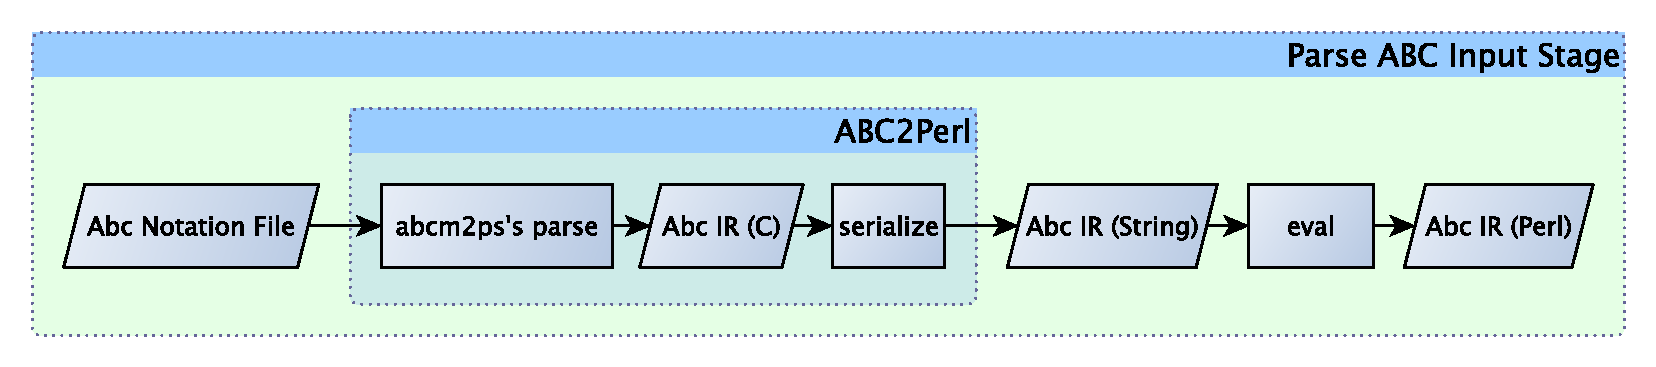
\includegraphics[width=\textwidth]{../img/parse_abc_input_stage.pdf}
  \end{figure}
\end{frame}

\note[itemize]{
\item O parser foi isolado e extraído do programa \abcmtops{}, um programa que gera partituras nos
formatos PostScript ou SVG.
\item É constante e independente da transformação pretendida, logo é comum a todas as ferramentas.
\item E a representação interna gerada é source-wise, ou seja, é uma lista de elementos cuja ordem é
igual ao \abc{} original. [NEXT]\\
\item Então, nesta fase de parsing é feita uma serialização Perl da estrutura gerada pelo parser do
\abcmtops{} (conseguida através do programa criado por mim, o ABC2Perl). Que depois é processada
através da função \emph{eval} do Perl transformado-a numa \emph{hash} Perl para ser transformada na
fase seguinte.
}

\begin{frame}{2) Transform the generated representation stage}
  \begin{itemize}
    \item IR's traversal, applying a rule-based transformation
    \pause
    \item Transformation specified as \abcdtrules{}
    \pause
    \item \abcdt{}'s main processor - \dt{}
  \end{itemize}
\end{frame}

\note{
A fase de transformação consiste em fazer uma travessia da representação gerada na fase de parsing e
aplicar-lhe uma transformação baseada em regras.

[NEXT]\\
A transformação a aplicar é especificada, em Perl, através de um conjunto de regras \abcdt{}.

[NEXT]\\
E a travessia é feita invocando o processador principal do \abcdt{}, chamado \dt{}, juntamente com
as regras.
}

\begin{frame}[fragile]{... \abcdtrules{}}
  \begin{block}{\abcdtrule{}}
    \emph{actuator} ⇒ \emph{transformation}
    \begin{itemize}
      \item \emph{actuator}: pattern for selecting an \abc{} element or a group of elements
      \item \emph{transformation}: instructions for processing an \abc{} element
    \end{itemize}
  \end{block}

  \pause
  \begin{exampleblock}{Actuator Examples}
    \begin{Verbatim}[fontsize=\footnotesize]
note
V:Tenor::note::_B
MIDI::channel
    \end{Verbatim}
  \end{exampleblock}

  \pause
  \begin{block}{Special Actuators}
    \begin{itemize}
      \item \emph{-default}: Describes how to transform unmatched \abc{} elements
      \item \emph{-end}: Enables a general post processing
    \end{itemize}
  \end{block}

\end{frame}

\note{
Uma regra \abcdt{} é uma correspondência entre um actuador e uma transformação. Um actuador consiste
num padrão para selecionar elementos \abc{} e uma transformação consiste num conjunto de instruções
para processar o elemento selecionado.

[NEXT]\\
Eis 3 exemplos de atuadores: o 1º seleciona qualquer nota, o 2º qualquer nota \texttt{si bemol} que
pertença à voz Tenor e o 3º qualquer comando \texttt{channel} que é um comando abcMIDI.

[NEXT]\\
Existem ainda dois actuadores especiais. O -default que descreve qual a transformação por defeito
para elementos que não façam match com nenhuma regra; e o -end que permite especificar um
processamento geral após a travessia.
}

\begin{frame}{... \abcdt{}'s main processor - \dt{}}
\pause
  \begin{algorithm}[H]
    \Begin{
      \KwIn{abc-file}
      \KwIn{rules: ($actuator \hookrightarrow transformation$)}
      $musicIR \gets eval($ abc2perl(abc-file) $)$ \hfill //1st stage\\
      \ForAll{$ elem \in musicIR $}{ \hfill //2nd stage\\
         $context \gets$ \mbox{\small{\texttt{recalculate current context}}}\\
         $transformation \gets$ \small{\texttt{rule\hspace{-0.1cm} ∈\hspace{-0.1cm}
         rules\hspace{-0.1cm} w/\hspace{-0.1cm} best\hspace{-0.1cm} matching\hspace{-0.1cm}
         actuator}}\\\hspace{3cm}\textbf{or} \mbox{\small{rules\{-default\}}}\\
         \hspace{3cm}\textbf{or} \mbox{\small{\toabc{}}}\\
         $res \gets$ \small{\emph{res ++ transformation(elem, context)}}\\
      }
      \Return{rules\{-end\} \textbf{or} $res$} \hfill //3rd stage\\
    }
  \end{algorithm}
\end{frame}

\note[itemize]{
\item A travessia da representação interna é feita invocando o processador \dt{}, cujo algoritmo é o
seguinte: [NEXT]
\item Recebe o ficheiro \abc{} e o conjunto de regras.

A 1ª fase é a de parsing onde é gerada a representação interna. Na 2ª fase (a de transformação) para
cada elemento da representação, o contexto é calculado. Também é extraída do conjunto de regras a
transformação cujo actuador faz melhor match com o elemento. Se nenhum atuador fizer match, a
transformação -default é extraída, e se essa também não tiver sido definida, então é utilizada a
função identidade, o \toabc{}. O resultado de cada transformação individual é concatenado ao
resultado anterior.

No final da travessia (a 3ª fase), se existir uma transformação -end o seu resultado é retornado,
caso contrário, é retornado o resultado da transformação calculada na fase 2).
}

\begin{frame}{3) Generate the output stage}
  \begin{itemize}
    \item Output generation of the transformation
    \pause
    \item String concatenation by default
    \pause
    \item Post processing for output transformation
  \end{itemize}
\end{frame}

\note{
Na última fase, como acabei de mencionar, é gerado um output da transformação realizada.

[NEXT]\\
Por omissão, a transformação aplicada a um elemento \abc{} é a função identidade, o \toabc{}, logo o
output final acaba por ser a concatenação de cada transformação individual.

[NEXT]\\
No entanto, o \abcdt{} permite que um pós-processamento seja feito no final da travessia, o que, por
sua vez, permite que se manipule o output final e se gere qualquer formato que se pretenda.
}

\begin{frame}{\abcdt{} by example}
  \begin{block}{\wcabc{}}
    Prints voices, measures and notes/pitches per voice counts for each ABC file
  \end{block}
  \pause
  \begin{block}{\wcabc{}'s algorithm}
    \begin{algorithm}[H]
      \Begin{
        \KwIn{abc\_tunes}
        \ForAll{$ tune \in abc\_tunes $}{
          $dt(tune,rules)$\\
        }
        $res \gets create\_output()$\\
        \Return{$res$}
      }
    \end{algorithm}
  \end{block}
\end{frame}

\note{
Nesta dissertação foram criadas algumas ferramentas utilizando o \abcdt{}.

[NEXT]\\
Uma delas foi o wc\_abc que, à semelhança do wc do \unix{}, gera um sumário com contagens, neste
caso, do número de vozes, compassos, notas e alturas por voz.

[NEXT]\\
O seu algoritmo consiste em processar cada música com o processador \dt{} para produzir as contagens
desejadas. No final, um output é gerado a partir das contagens recolhidas.
}

\begin{frame}[fragile]{\abcdt{} by example}
  \begin{block}{\abcdtrules{} for \wcabc{}}
  \begin{center}
  \begin{tabular}{|p{2cm}|p{5cm}|}
    \hline
    Actuator & Transformation (Perl)\\
    \hline
    \hline
    \emph{V:} & \small{\texttt{voice\_count++;}}
    \\
    \hline

    \hline
    \emph{note} & \small{\texttt{note\_count\{voice\}++; pitch\_count\{voice\}++;}}
    \\
    \hline

    \hline
    \emph{bar} & \small{\texttt{measure\_count\{voice\}++;}}
    \\
    \hline
  \end{tabular}
  \end{center}
  \end{block}
\pause
  \begin{block}{Excerpt of \wcabc{}'s output}
    \lstinputlisting[basicstyle=\footnotesize]{wc_abc_output.tex}
  \end{block}
\end{frame}

\note[itemize]{
\item As regras \abcdt{} para o cálculo das contagens são estas. Do lado esquerdo estão os
actuadores e no direito as respetivas transformações. Para facilitar a leitura, o código Perl foi
passado para dentro de funções, cujo nome ajuda a perceber a ação semântica.
\item Portanto, o número de vozes é incrementado quando o elemento voz é visitado e este é a
primeira vez que que surge na música.
\item O número de notas e alturas são incrementados quando uma nota é visitada.
\item E o número de compassos é incrementado quando uma barra de compasso é visitada.
\item NEXT Isto é um excerto de um  output exemplo gerado pelo \wcabc{}
}

\begin{frame}{\abcdt{} by example}
  \begin{block}{paste\_abc}
    Merges voices parallel to each other in the time perspective.
  \end{block}
  \begin{block}{cat\_abc}
    Concatenates scores one after the other in the time perspective.
  \end{block}
  \begin{block}{learning\_abc}
    Generates two \abc{} scores whose goal is to help musicians in individual rehearsal of
    multi-voice music.
  \end{block}
  \begin{block}{detect\_errors\_abc}
    Detects syntactical errors in an \abc{} score and warns the user.
  \end{block}
  \begin{block}{find\_chords\_abc}
    Searches melodically expressed chord formations.
  \end{block}
\end{frame}

\note[itemize]{
\item As outras ferramentas criadas são:
  \item O paste\_abc junta vozes paralelamente na perspectiva temporal.
  \item O cat\_abc concatena músicas umas a seguir às outras na perspectiva temporal.
  \item O learning\_abc gera dois ficheiros \abc{} cujo objectivo é auxiliar músicos no estudo
  individual de música multi-voz. Um realça uma voz e o outro realça as restantes.
  \item O detect\_errors\_abc deteta erros sintáticos num ficheiro \abc{} e gera mensagens de erro
  para o utilizador.
  \item O find\_chords\_abc procura formações de acordes expressos melodicamente.
}

\begin{frame}[fragile]{\abcdt{} by example}
  \begin{block}{canon\_abc}
    Generates a complete canon score from a set of \abc{} files containing the melodic parts and,
    optionally, the accompaniment part.
  \end{block}
  \begin{exampleblock}{Usage}
    \textbf{canon\_abc} \emph{violini.abc+8 violini.abc+16 violini.abc+24 basso.abc++}

    \begin{figure}[H]
      \begin{center}
        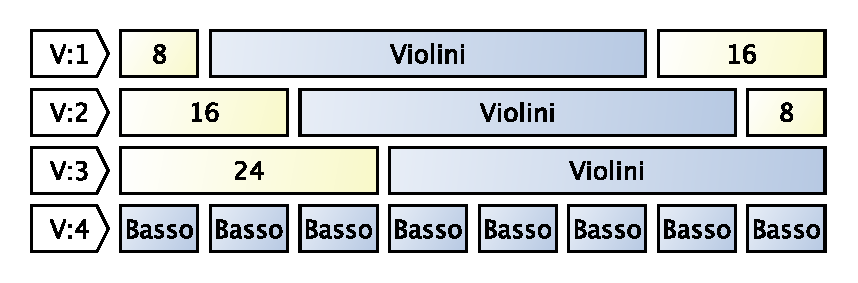
\includegraphics[width=0.8\textwidth]{../img/pcanon_scheme.pdf}
      \end{center}
    \end{figure}
  \end{exampleblock}
\end{frame}

\note[itemize]{
  \item O canon\_abc gera um canon completo a partir de um conjunto de ficheiros \abc{} que contêm
  as partes melódicas e, opcionalmente, a parte de acompanhamento.
  \item Por exemplo, para gerar o Canon de Pachelbel, invoca-se o comando desta forma, passando as
  partes melódicas com o desfasamento pretendido para cada voz e identifica-se a parte de
  acompanhamento. É então gerada uma música com esta estrutura.
}

\begin{frame}{Conclusions}
  \begin{itemize}
    \item The \unix{} philosophy was a major influence for the conception of this work
    \item Reusing \abcmtops{}' parser was very important to help guarantee this work's quality,
    coverage and developing time
    \item \abcdt{} considerably simplifies the process of creating compact \abcpt{}s
    \item Perl provides a rich environment to allow easy processing of text and a bigger expressive
    power to specify transformations
    \item \emph{http://search.cpan.org/dist/Music-Abc-DT/}
  \end{itemize}
\end{frame}

\note[itemize]{
\item A filosofia \unix{} e as suas ideias simples e bem sucedidas foram uma influência enorme na
conceção deste trabalho.
\item A reutilização do parser do \abcmtops{} foi importante para garantir a qualidade, abrangência
e tempo de desenvolvimento deste trabalho.
\item O \abcdt{} simplifica consideravelmente o processo de criação de ferramentas que processem
\abc{}
% , já que 1) não é necessário especificar aquilo que não precisa de ser transformado, 2) a
% utilização de regras facilita a escrita das transformações e 3) existe um conjunto rico de atuadores
% que permite selecionar pontos específicos para transformar.
\item Utilizar o Perl como linguagem embutida no \abcdt{}, proporciona um ambiente rico para
processar texto. Além disso, estruturas como hashes dão um maior poder expressivo para especificar
transformações.
}

\begin{frame}{Future Work}
  \begin{block}{Internal Representation}
    A more throrough investigation on music representation
  \end{block}
  \begin{block}{Musical Corpora}
    Build a rich \abc{} corpus\\
    Develop statistical models
  \end{block}
  \begin{block}{\abcdt{}}
    Expand set of actuators and default functions\\
    Study another actuator specification's approach
  \end{block}
  \begin{block}{Toolkit}
    Develop new tools\\
    Improve existing ones
  \end{block}
\end{frame}

\note[itemize]{
\item Na área da IR, far-se-á uma investigação mais completa sobre representação
de música para obter um ambiente que consiga responder mais facilmente a tarefas mais específicas.
\item Na área do corpus musical, construir-se-á um corpus de \abc{} para servir como material de
teste para o toolkit e para treinar sistemas de aprendizagem;
\item E desenvolver-se-á um conjunto de modelos estatísticos para obter funcionalidades como a
classificação de obras e geração de música;
\item No \abcdt{}, o conjunto existente de atuadores e funções pré-definidas será expandido;
\item E outra abordagem para a especificação de atuadores será estudada.
\item Novas ferramentas \abc{} serão desenvolvidas e adicionadas ao toolkit
\item e as ferramentas existentes serão aperfeiçoadas.
}

\begin{frame}[plain]
	\begin{center}
	\maketitle
	\end{center}
\end{frame}

\begin{frame}{References}
	\begin{thebibliography}{1}
  \bibitem{Azevedo2013} Bruno Azevedo and José João Almeida, "ABC with a UNIX Flavor," \textit{Symposium on Languages, Applications and Technologies}, 29, 2013.
  \end{thebibliography}
\end{frame}

\end{document}
